Here is all the stuff of the analysis!

\section{Final state particle}
	-final state particle: proton, antiproton, \piminus, \piplus, \kminus and \kplus mesons
	
	-reconstructed in Detector
	
	-only particles with more then 3 hits either in one of the subdetectors (reason: 3 hits define circle; fourth hit point gives a validation for track hypothesis)
	
	- ideal PID (reason!!!)
	
	-reco efficiency in table \ref{tab:finalstate_recoeff}
	
	\begin{table}
		\centering
		\caption{reco efficiency and momentum resolution}
		\label{tab:finalstate_recoeff}
		\begin{tabular}{lll}
			\hline
			final state & N/$\%$ & $\frac{\sigma p}{p}/\%$ \\
			\hline
			\hline
			\piminus &  & \\
			\piplusone(\anticascade) &  & \\
			\piplustwo(\alam) &  &\\
			\kminus&  &\\
			p &  &\\
			\antiproton &  &\\\hline
			 
		\end{tabular}
	\end{table}
	

	
\section{Reconstruction of $\boldmath{\Lambda}^0$ and $\boldmath{\bar{\Lambda}^0}$}
	\subsection{Combination}
		-only final state particle with more than 3 Hits
		
		-daughter particles for \lam: proton an \piminus meson
		
		-daughter particles for \alam: \antiproton and \piplus here \piplustwo 
		
		-for c.c. chain: \lam: proton and \piminustwo; \alam: \antiproton and \piplus 
		
		-performing a mass window cut with width of $0.3$\massunit 
		
		
	\subsection{Fitting}
	
		- fitting particles to common vertex with PndKinVtxFitter
	
		- $\chi^{2}$ and $\chi^{2}$-Probability distiribution shown in figure \ref{fig:lambda_chi2}
		
		\begin{figure}
			\centering
				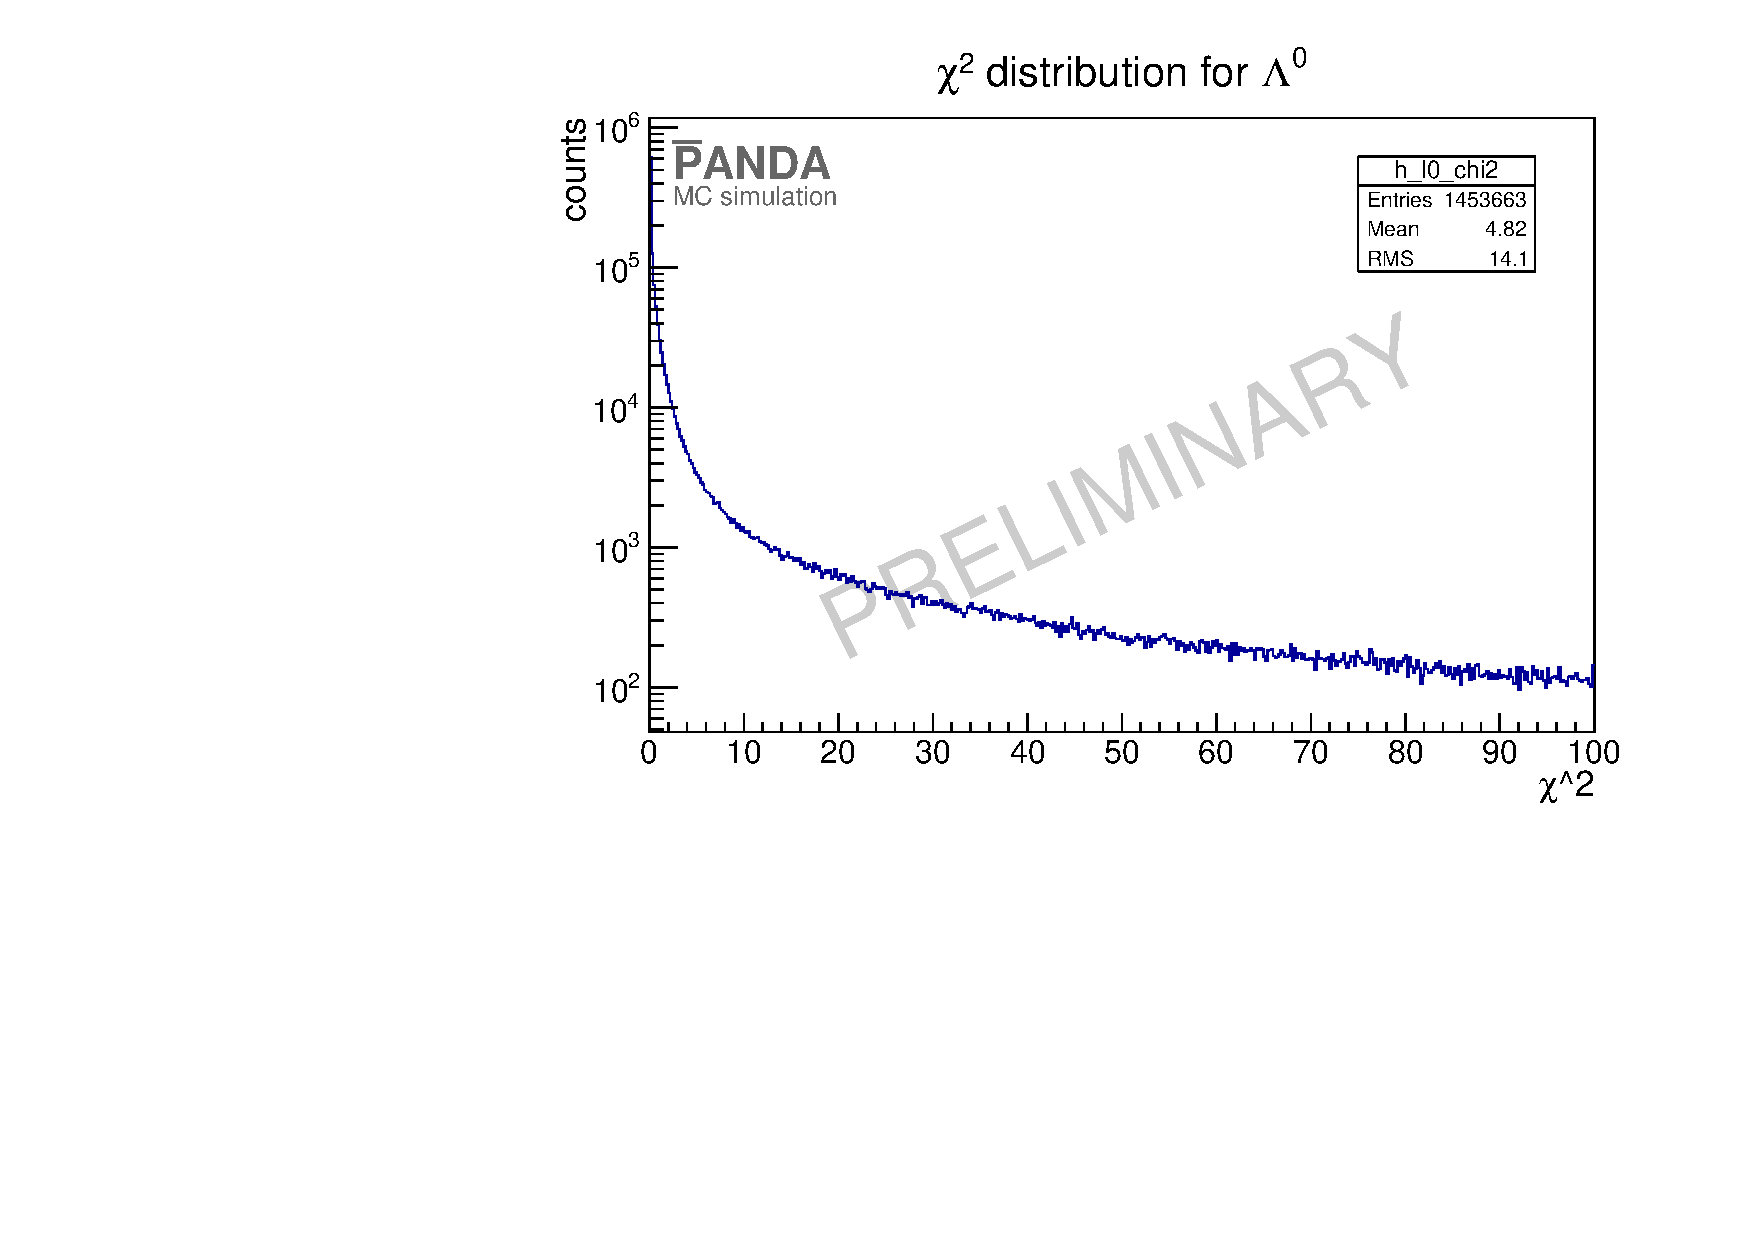
\includegraphics[width=0.50\textwidth]{./plots/lambda0/lambda0_chisqrt.pdf}
				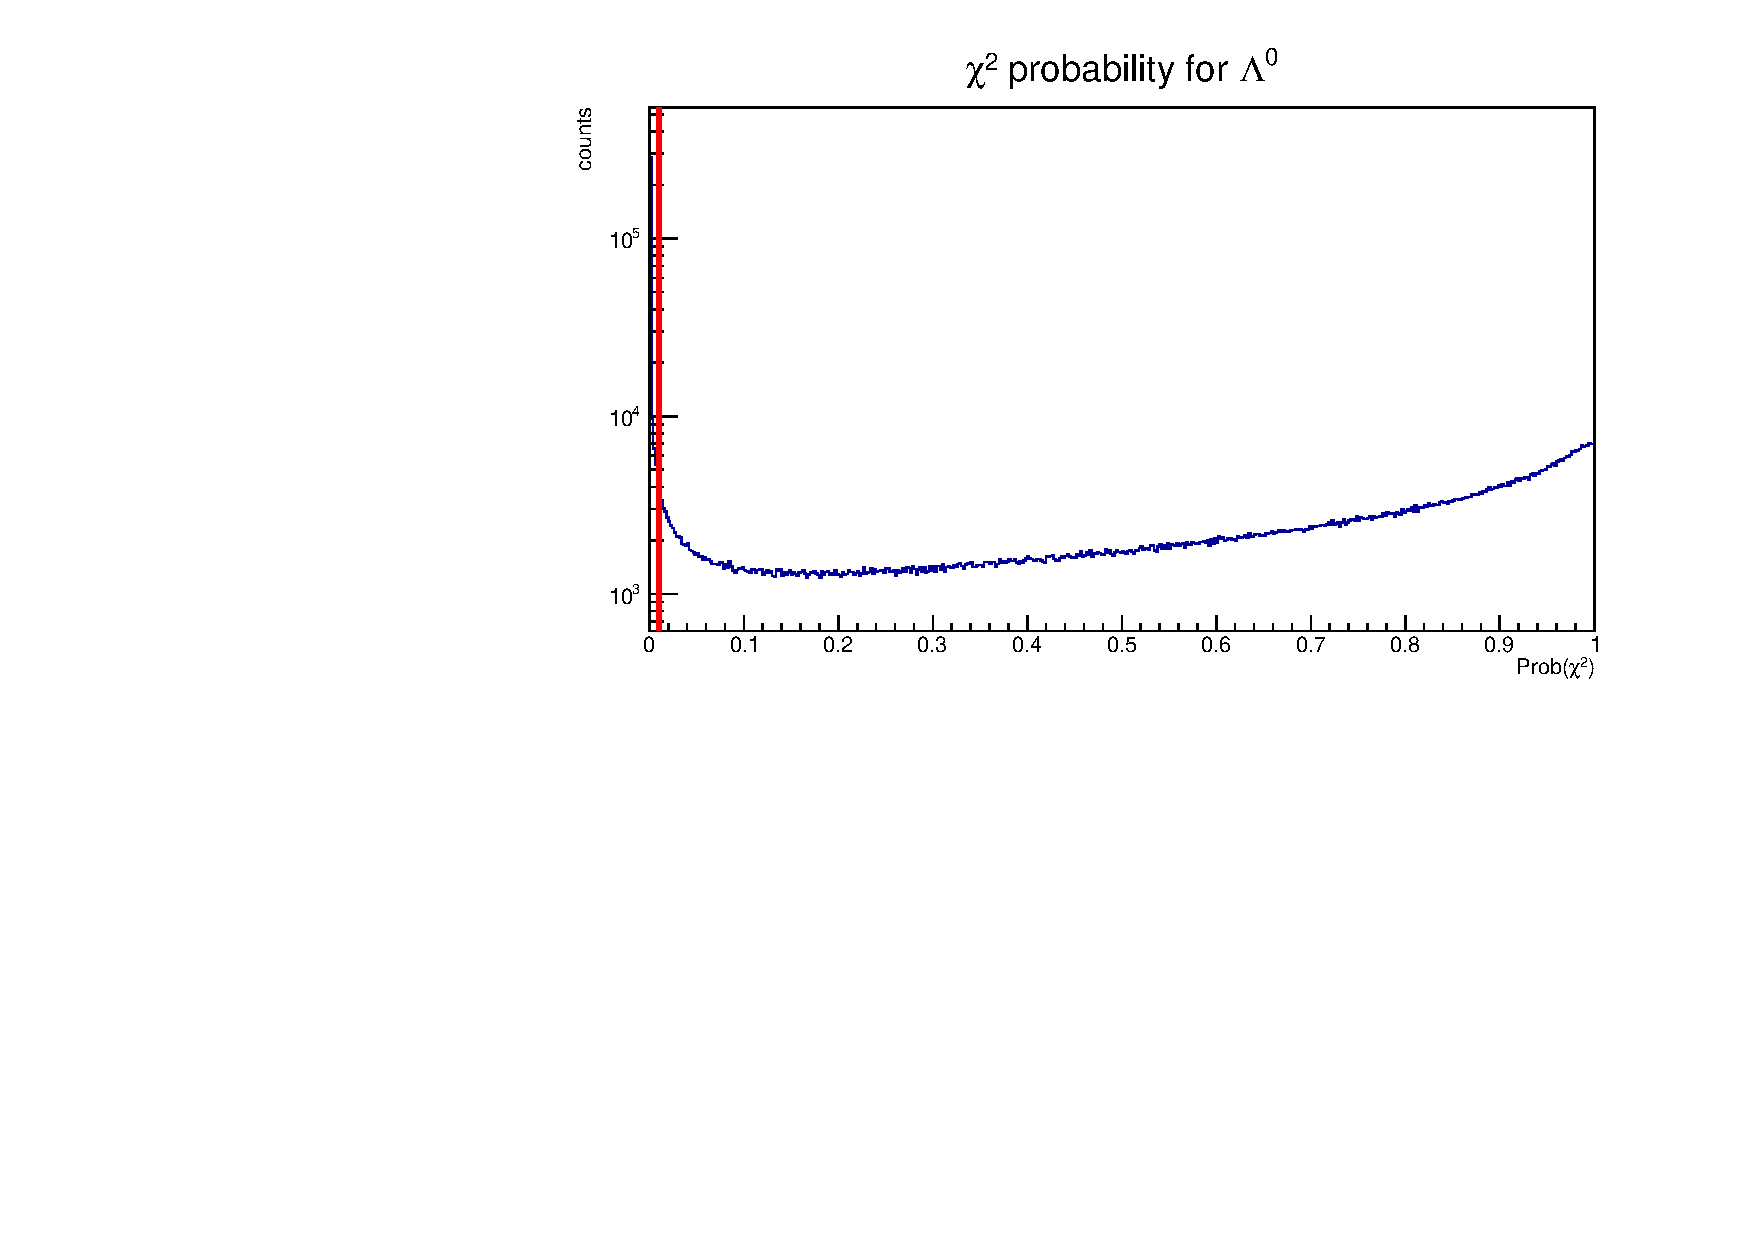
\includegraphics [width=0.50\textwidth]{./plots/lambda0/lambda0_prob.pdf}
			\caption{upper: $\chi^{2}$ distribution; lower: $\chi^{2}$ probability distribution}
			\label{fig:lambda_chi2}
		\end{figure}
		
		- features in probability distribution are not coming from vertex fitting. There is still a problem with covariance matrices.
		
		- fit information are given to PndKinFitter with mass constraint
		
		- only select particles with prob bigger than 0.01 for both fitters
		
		- scheme in figure \ref{fig:lambda_scheme}
		
		\begin{figure}
			\centering
				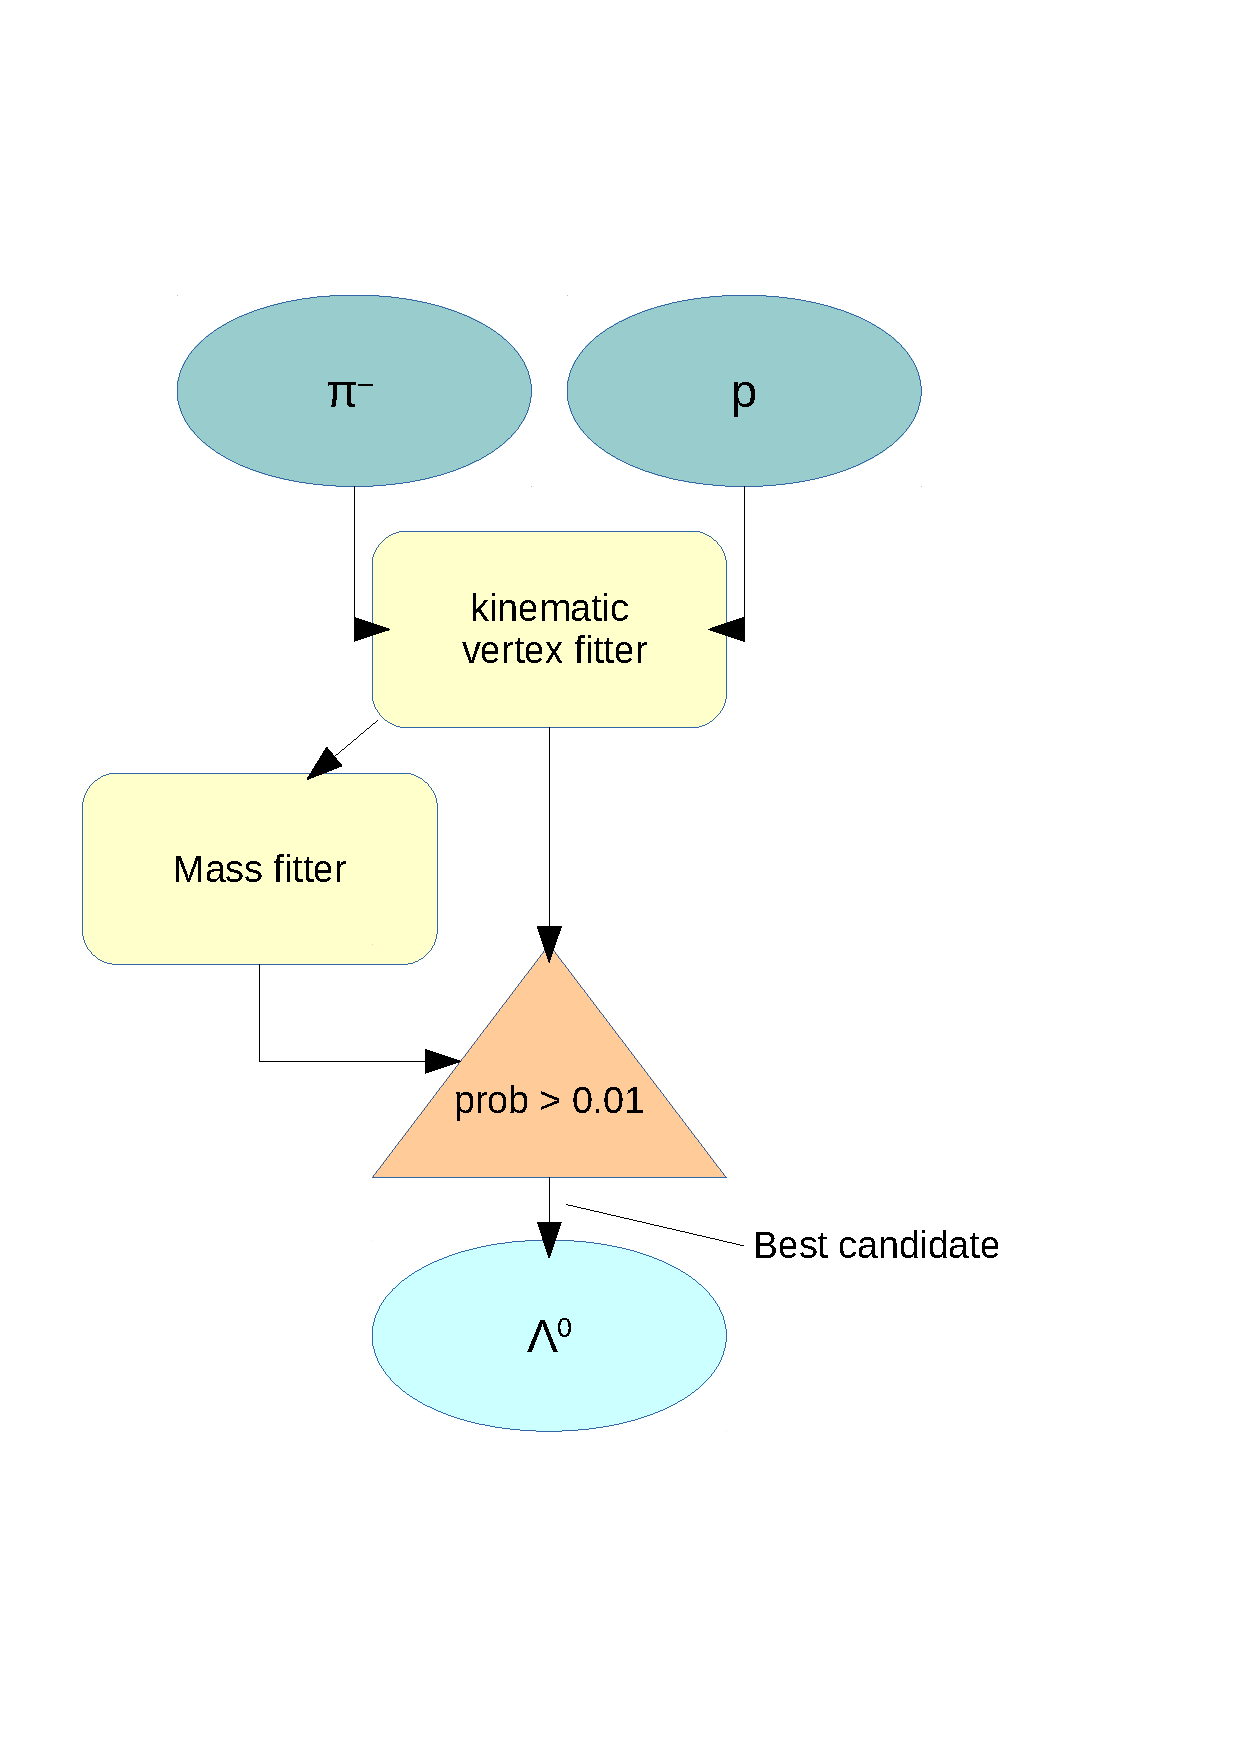
\includegraphics[width=0.50\textwidth]{./plots/combineLambda0.pdf}
			\caption{Scheme for \lam reconstruction}
			\label{fig:lambda_scheme}
		\end{figure}
		
		-if there is more than one particle, choose best candidate
		
	\subsection{Results}
	
		- mass distribution for different cuts see figure \ref{fig:lambda0_massdiffcuts} and figure \ref{fig:antilambda0_massdiffcuts}
		
		\begin{figure}
			\centering
				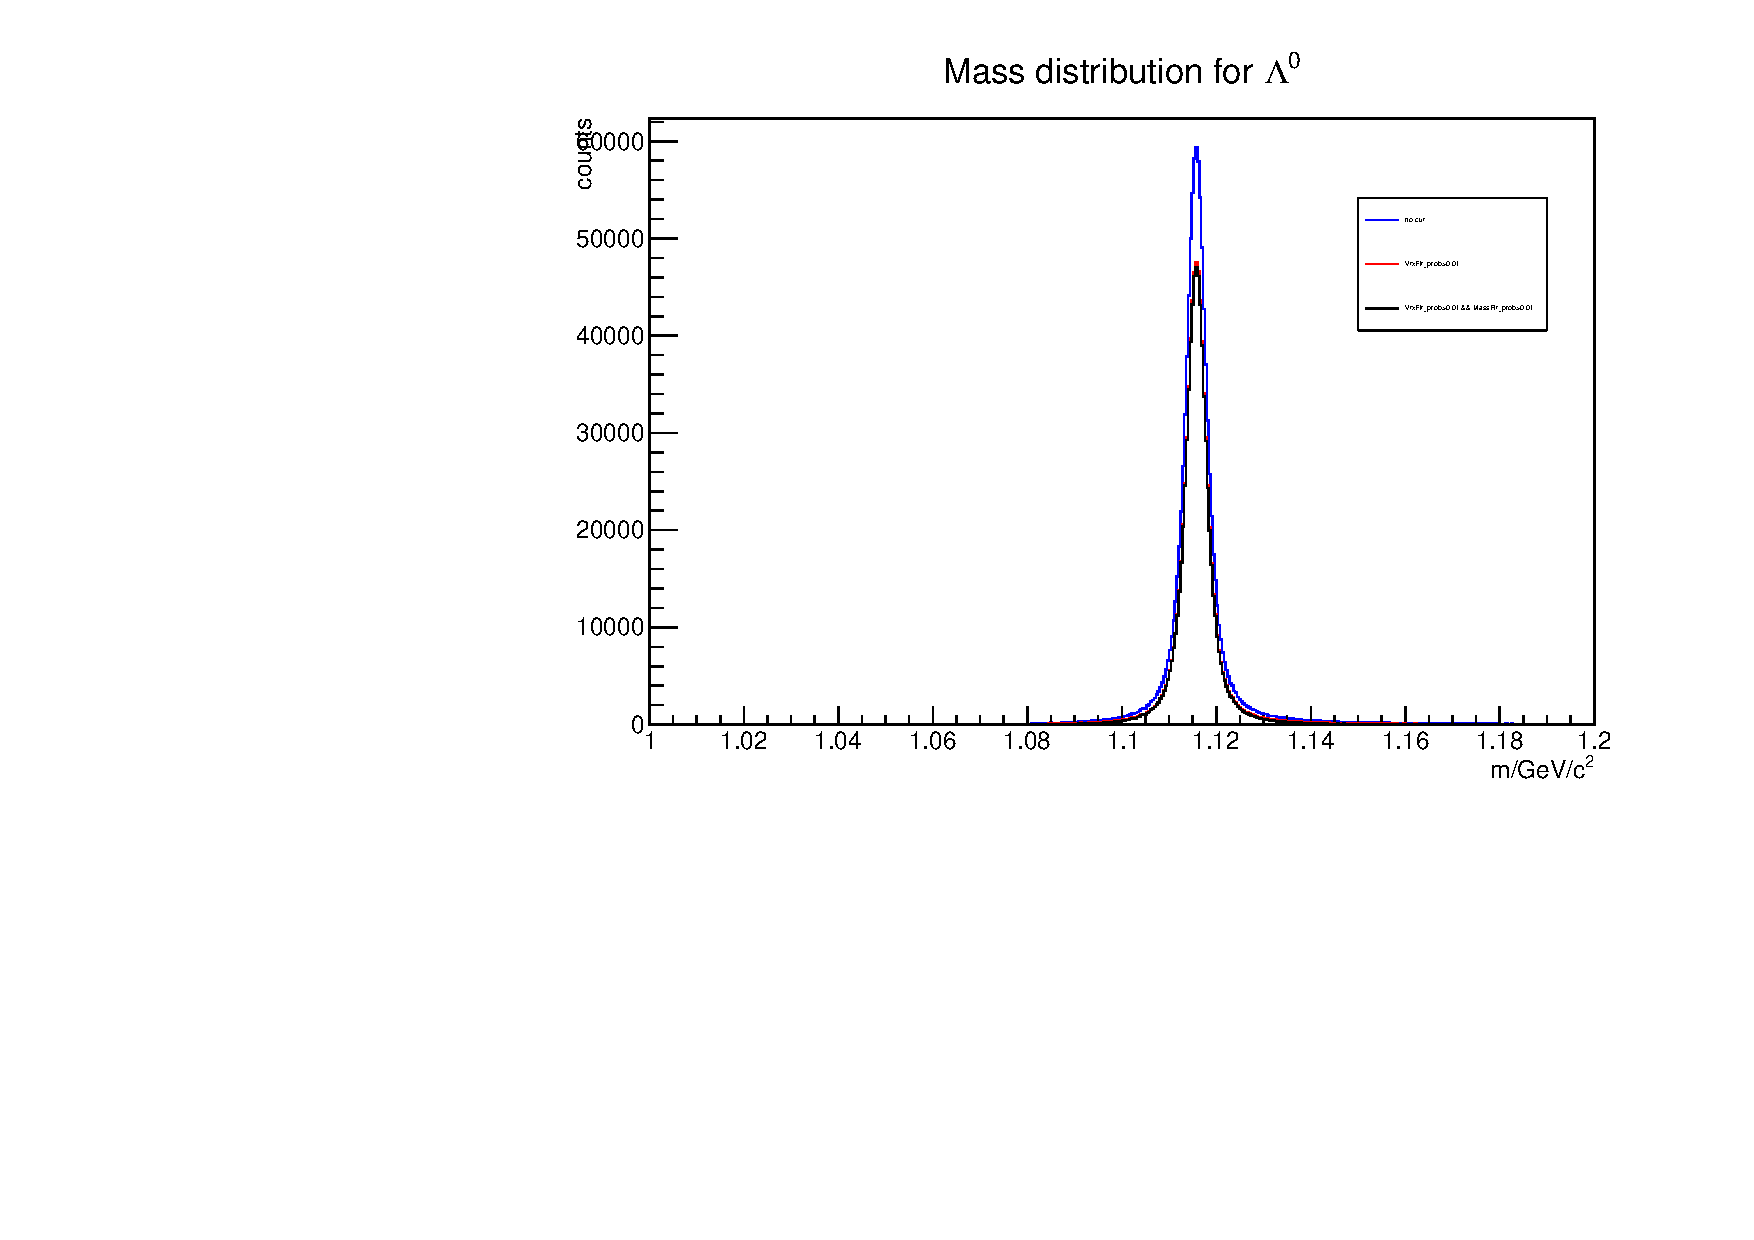
\includegraphics[width=1.1\textwidth]{./plots/lambda0/lambda0_m_diffcuts.pdf}
			\caption{Mass distribution of \lam for different cuts}
			\label{fig:lambda0_massdiffcuts}
			
				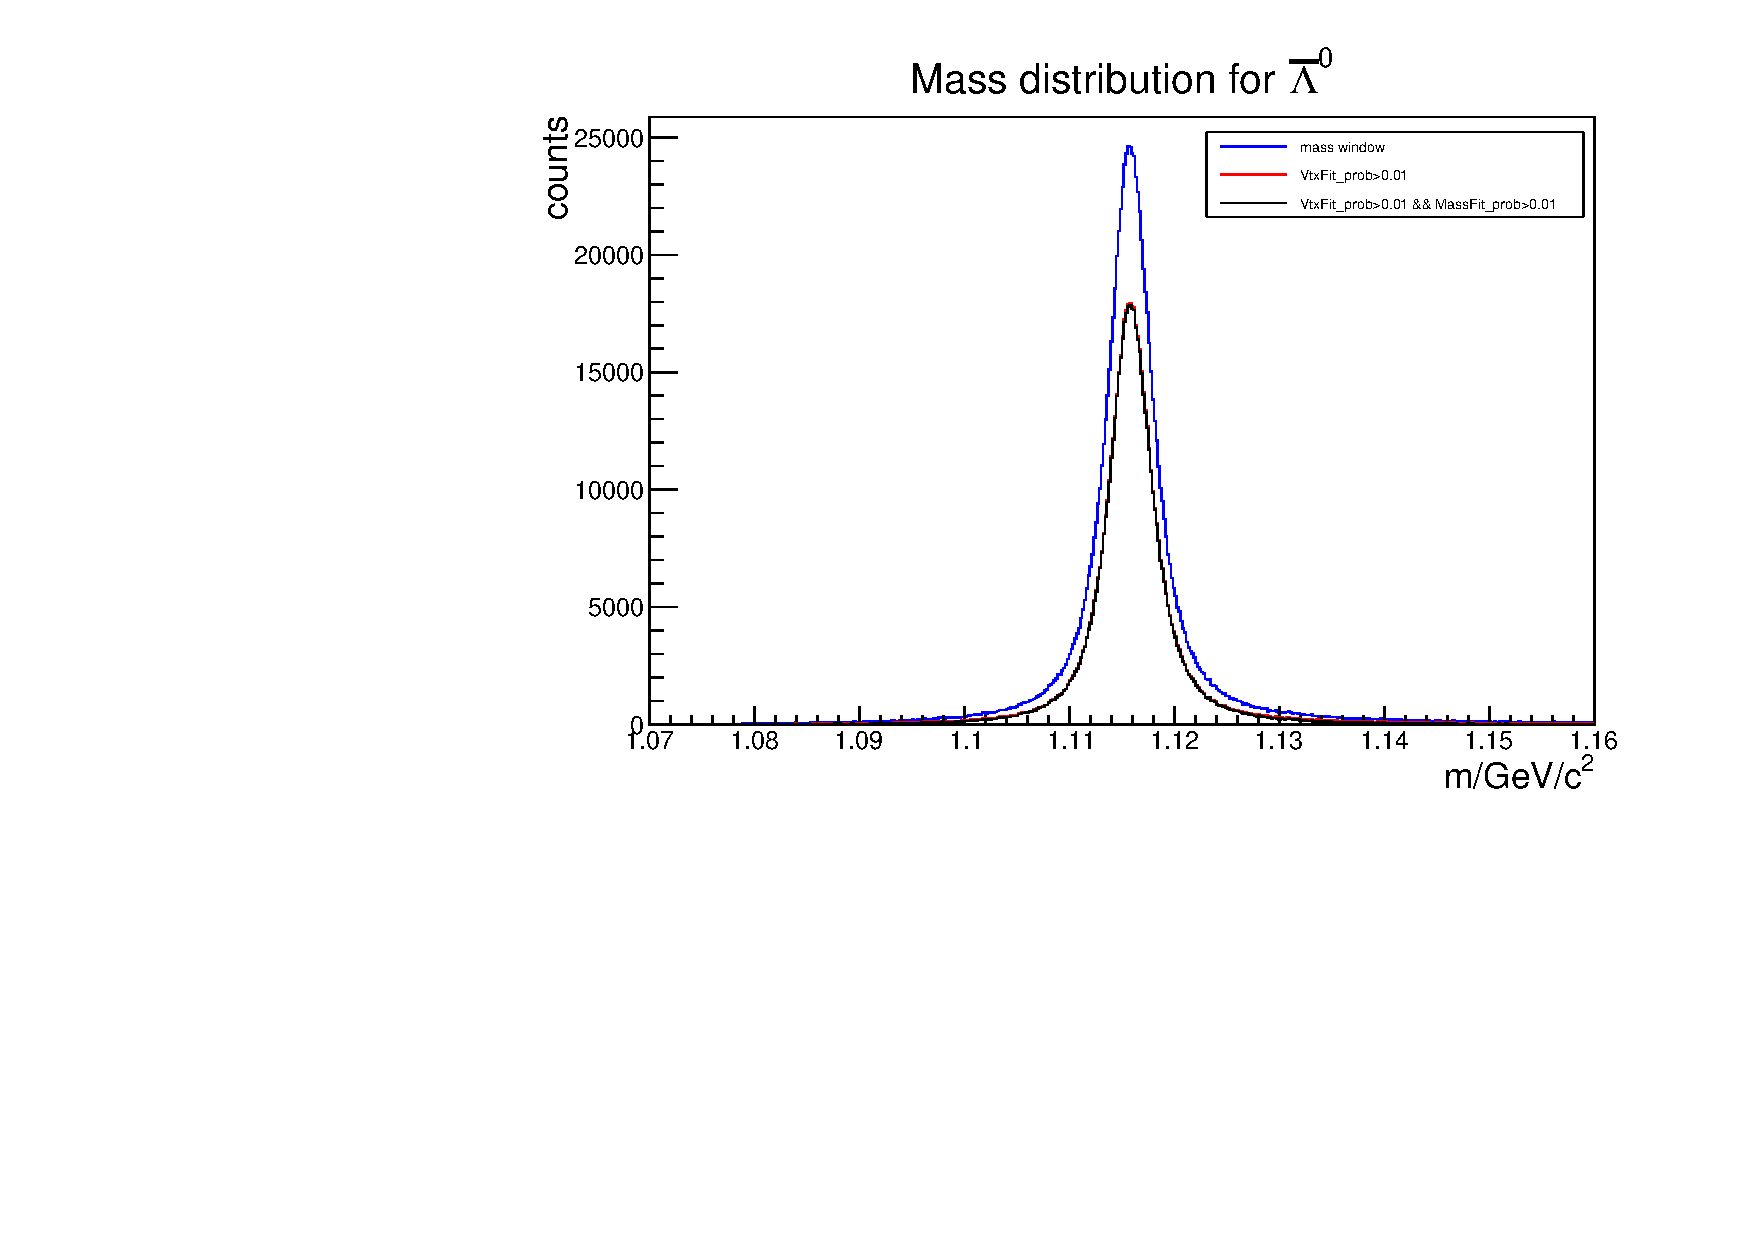
\includegraphics[width=1.1\textwidth]{./plots/antilambda0/antiLambda0_m_diffcuts.pdf}
			\caption{Mass distribution of \alam for different cuts}
			\label{fig:antilambda0_massdiffcuts}
		\end{figure}
		
		-performing a doulbe gaussian fit on cutted mass for \lam and \alam (example see figure \ref{fig:lambda0_massfit}
		
		\begin{figure}
			\centering
				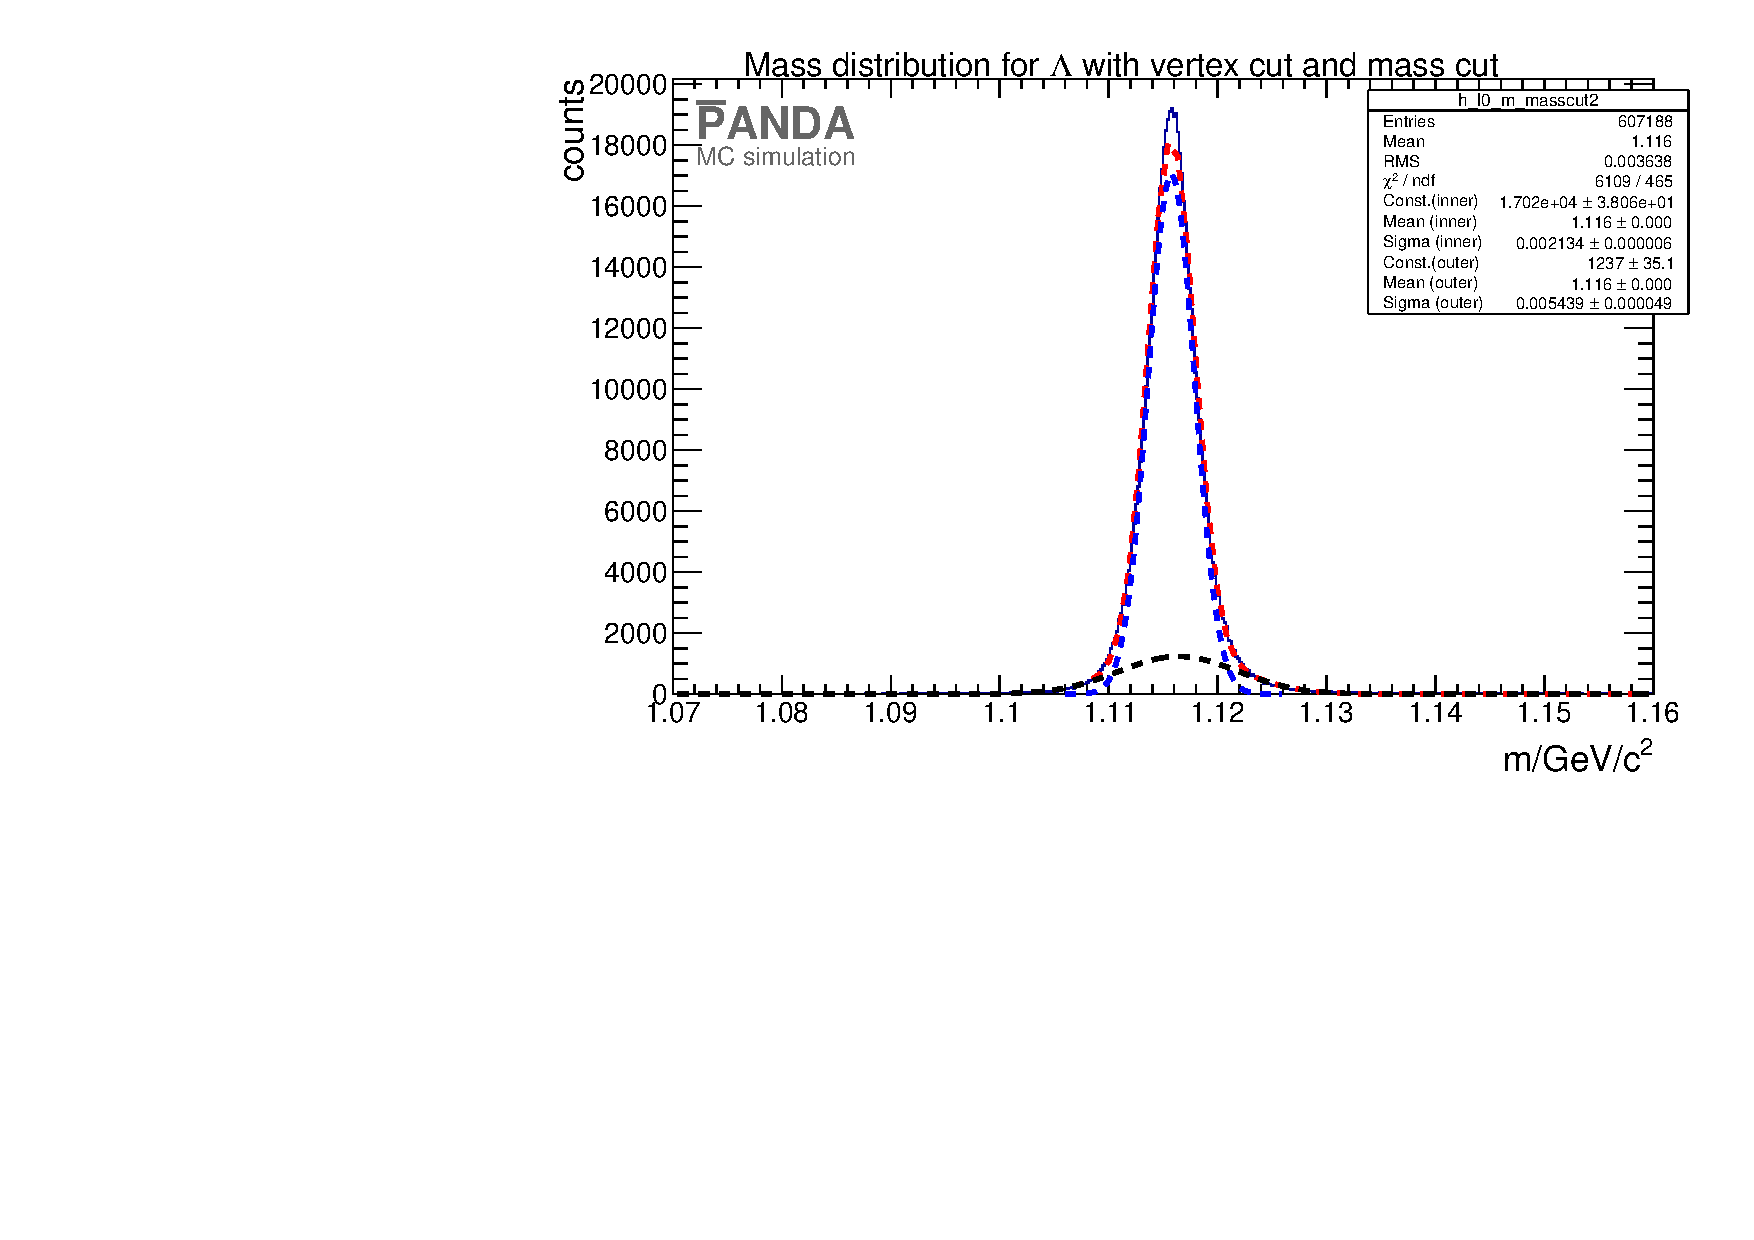
\includegraphics[width=0.8\textwidth]{./plots/lambda0/lambda0_m_masscut2.pdf}
			\caption{Mass fit with a double gaussian fit}
			\label{fig:lambda0_massfit}
		\end{figure}
		
		- result of massfit $\mt{m} = \left(1.116 \pm 0.002\right)$ \massunit
	
\section{Reconstruction of $\boldmath{\Xi}$ and $\boldmath{\bar{\Xi}}$}
	\subsection{Combination}
	
		-similar scheme for \lam and \alam
		
		-daughter particles for \anticascade: \antiproton and \piplus here \piplusone
		
		-daughter particles for \cascade:  \lam and \piminus meson here \piplusone
		
		-using best candidate from \lam and \alam
		
		-\piplus and \piminus with more than 3 Hits in one subdetector 
		
		-performing a mass window cut with width of $0.3$\massunit 
		
		
	\subsection{Fitting}
	
		- fitting particles to common vertex with PndKinVtxFitter
		
		- fit information are given to PndKinFitter with mass constraint
		
		- only select particles with prob bigger than 0.01 for both fitters
		
		- scheme in figure \ref{fig:anticascade_scheme}
		
		\begin{figure}
			\centering
				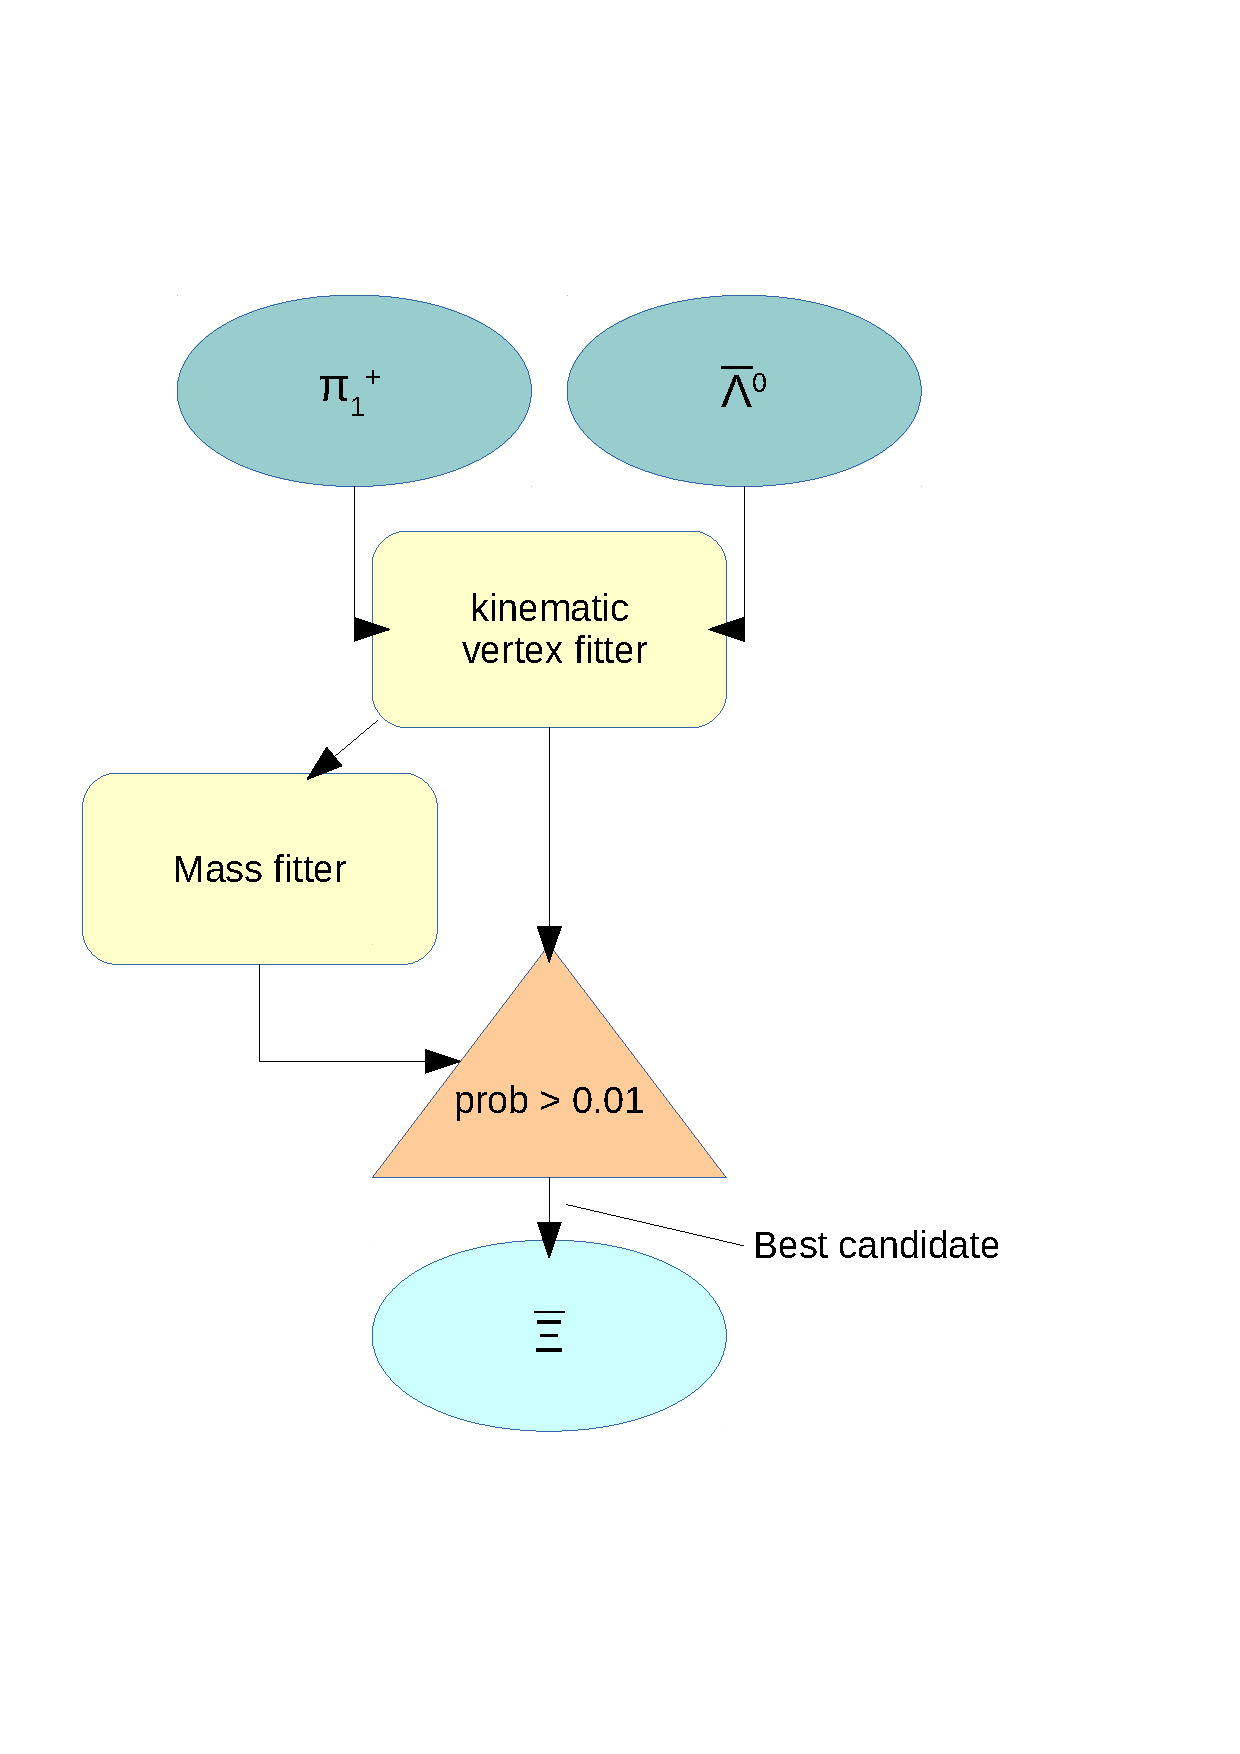
\includegraphics[width=0.50\textwidth]{./plots/combineAntiCascade.pdf}
			\caption{Scheme for \anticascade reconstruction}
			\label{fig:anticascade_scheme}
		\end{figure}
		
		-if there is more than one particle, choose best candidate

\section{Reconstruction of $\boldmath{\Xi}$(1820) and $\boldmath{\bar{\Xi}}$(1820)}
		\subsection{Combination}

		
		-daughter particles for \excitedcascade: \lam and \kminus meson
		
		-daughter particles for \excitedanticascade: \alam and \kplus 
		
		-using best candidate from \lam and \alam
		
		-\kplus and \kminus with more than 3 Hits in one subdetector 
		
		-performing a mass window cut with width of $0.3$\massunit 
		
		
	\subsection{Fitting}
	
		- fitting particles to common vertex with PndKinVtxFitter
		
		- fit information are given to PndKinFitter with mass constraint
		
		- only select particles with prob bigger than 0.01 for both fitters
		
		- scheme in figure \ref{fig:excitedcascade_scheme}
		
		\begin{figure}
			\centering
				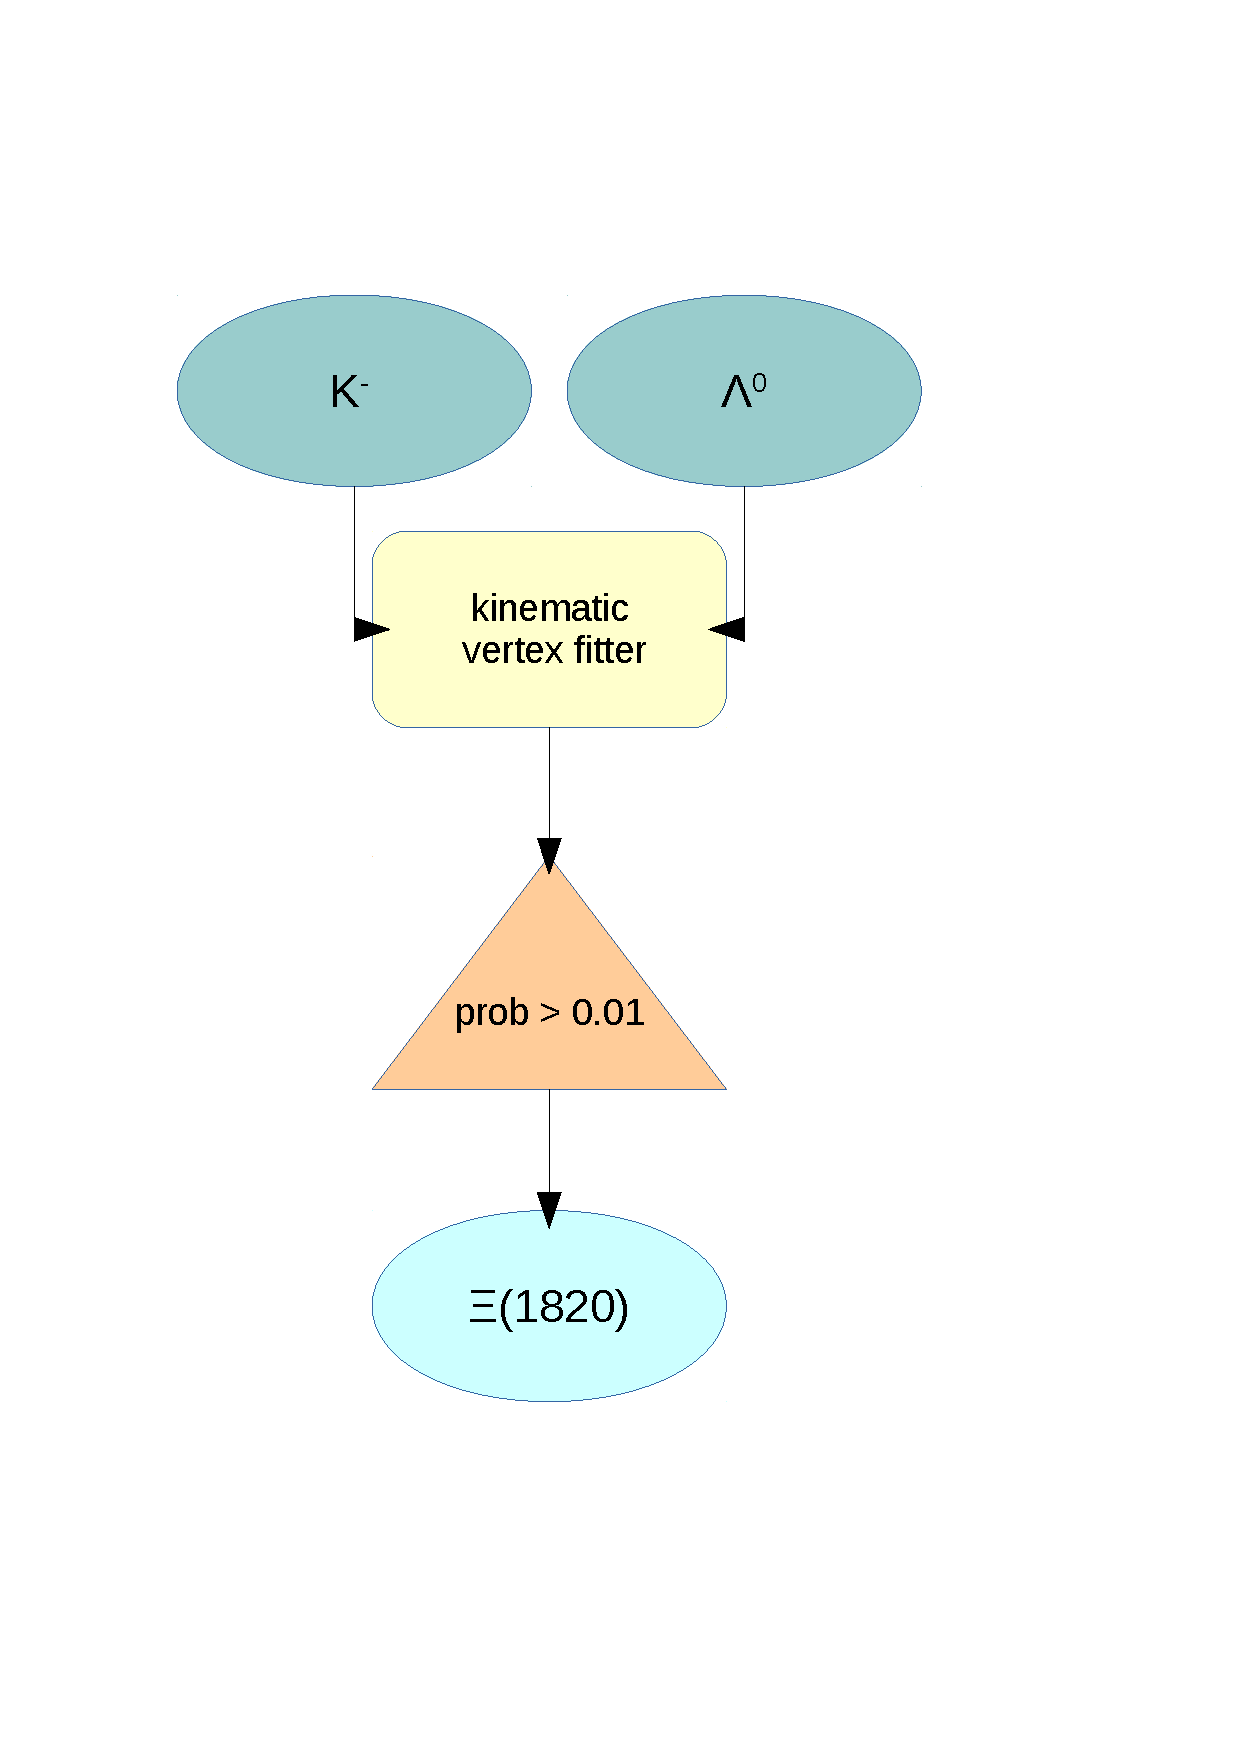
\includegraphics[width=0.50\textwidth]{./plots/combineExcitedCascade.pdf}
			\caption{Scheme for \excitedcascade reconstruction}
			\label{fig:excitedcascade_scheme}
		\end{figure}
		
		-if there is more than one particle, choose best candidate
	
\section{Reconstruction of hole chain}

	\subsection{combination}
	
	-using best candidate from \excitedcascade and \anticascade
	
	-for c.c : \excitedanticascade and \cascade
	
	-mass window of $0.3$\massunit
	
	
	\subsection{Fitting}
	
	-use PndKinFitter with four momentum constrained
	
	-initial four momentum vector is 
	\begin{center}
		\begin{equation}\nonumber
			\left(\mt{p}_x,\, \mt{p}_y,\, \mt{p}_z,\, \mt{E} \right) = \left(0,\, 0,\, 4.6,\, 5.63 \right)
		\end{equation}
	\end{center}
	
	
	-if probability is better than $1\%$ keep candidate
	-scheme shown in figure \ref{fig:fourconstraintfit}
	
	\begin{figure}
		\centering
			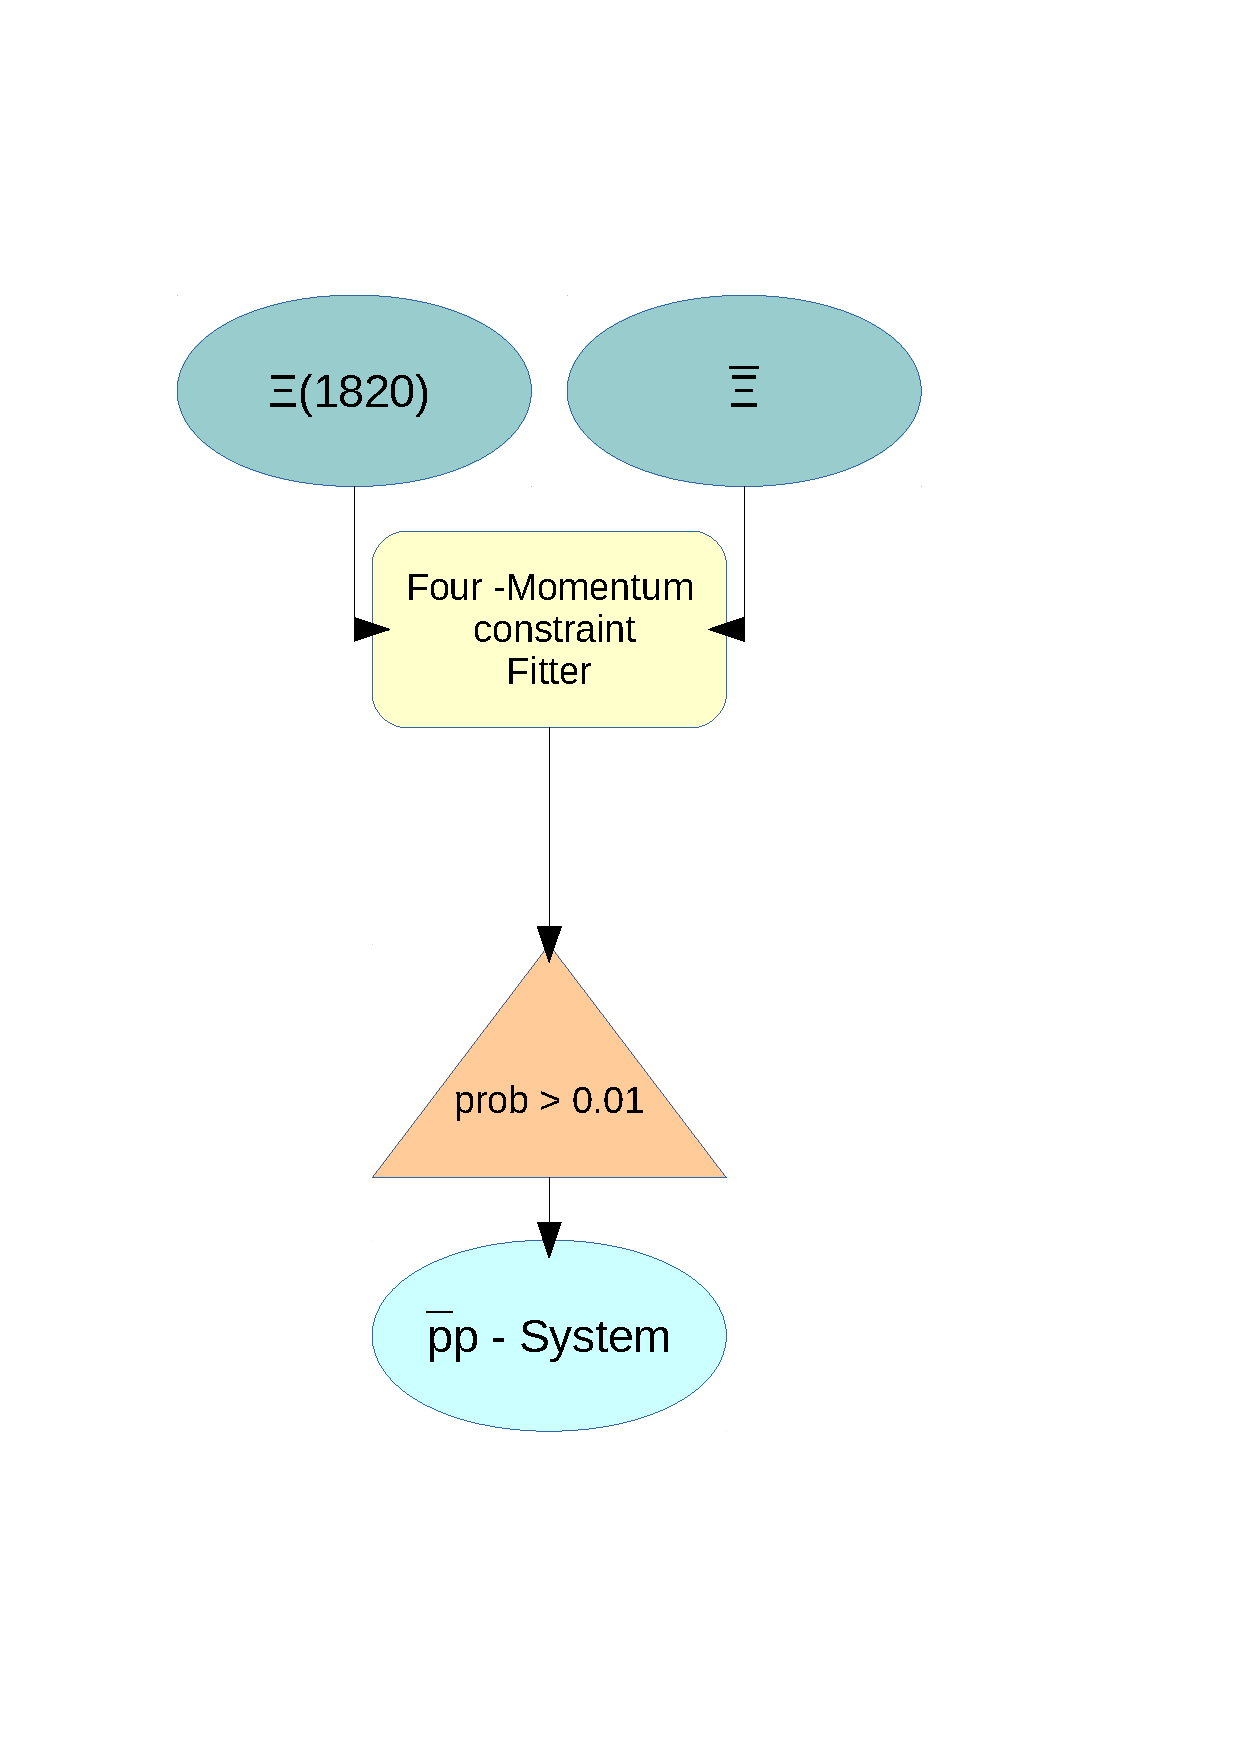
\includegraphics[width=0.50\textwidth]{./plots/combineCascadeSys.pdf}
		\caption{Scheme for 4-Constraint Fit}
		\label{fig:fourconstraintfit}
	\end{figure}